\documentclass[10pt,a4paper,notitlepage]{report}
\usepackage[utf8]{inputenc}
\usepackage{amsmath}
\usepackage{amsfonts}
\usepackage{amssymb}
\usepackage{graphicx}
\usepackage{xcolor}
\usepackage{geometry}
\usepackage{picins}
\geometry{a4paper, top=15mm, left=25mm, right=25mm, bottom=25mm, headsep=10mm, footskip=10mm}
\pagestyle{empty} %keine Kopf-/Fußzeile
\author{Sausage Pan}
\begin{document}
	%Farbdefinierung
	\definecolor{orange}{HTML}{F67800}
	\definecolor{hellorange}{HTML}{FFAD41}
	\definecolor{schwarz}{rgb}{0,0,0}
	%Stildefinitionen!!Wichtig!!
	\newcommand{\Eins}[1]{\color{orange}\textbf{{\Large#1}}} %Überschrift 1. Ordnung
	\newcommand{\Zwei}[1]{\color{orange}\textbf{{\large#1}}} %Überschrift 2. Ordnung
	\newcommand{\Drei}[1]{\color{orange}{\normalsize#1}} %Überschrift 3. Ordnung
	\newcommand{\Text}{\color{schwarz}} %normaler Fließtext
	\newcommand{\Fusszeile}
	{\textit{{\footnotesize Eckert, Georg - Roscher, Philipp - Krien, Alexandra - Sinakow, Sergej - Blasberg, Bettina - Groß, Stephanie Sara}}} %Fußzeile immer am Ende der Seite einfügen!
	%Randstreifen
	\marginpar{\vspace{3.0mm} \color{orange}\rule{0.8mm}{53.3mm} \\[3mm] \color{hellorange}\rule{0.8mm}{170mm}}
	%Header-Bild
	\begin{center}
		
\includegraphics[width=160mm]{header2}
	\end{center}
	%Eigentlicher Inhalt :D
	\Eins{Layoutentwürfe}\\
	\\
	\\
	\Zwei{Startbildschirm}\\
	\\
	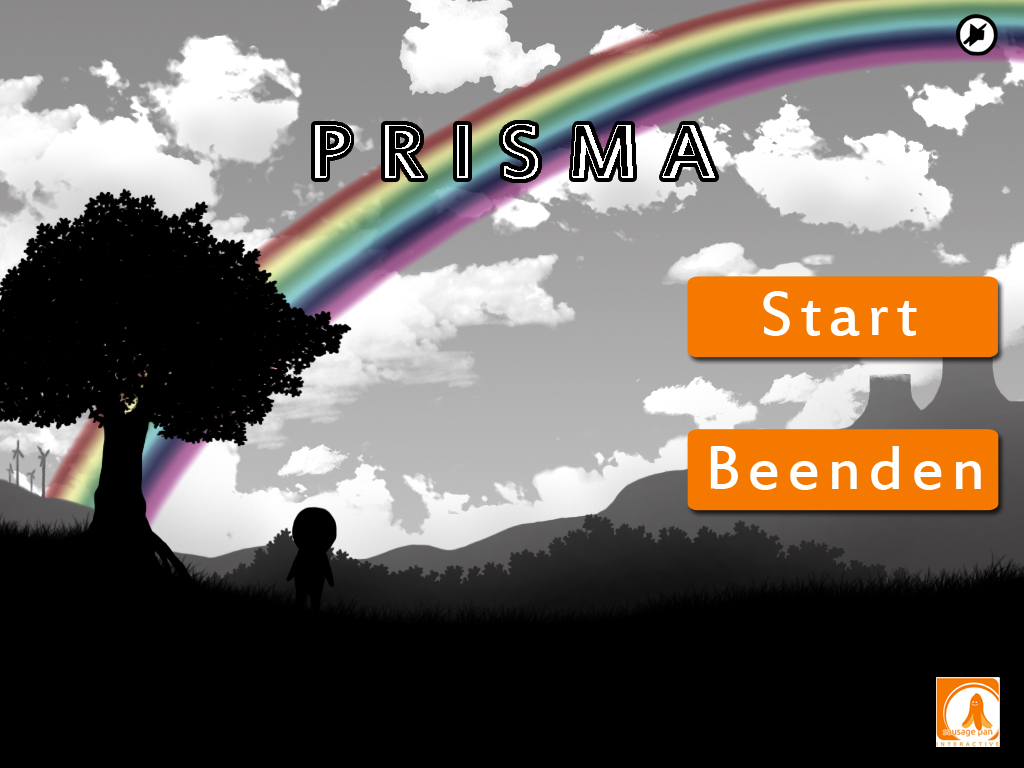
\includegraphics[width=1\textwidth]{png/startbildschirm.jpg}\
	\\\\
	\Text
	Hier zu sehen der Starbildschirm über den das Spiel begonnen wird. Der Hintergrund orientiert sich dabei stark an der Story des Spiels.\\
	Dies ist lediglich ein Entwurf zum generellen Konzept, der Schriftzug des Titels wird später sicherlich noch überarbeitet werden, er sei hier nur stellvertretend zu 		sehen.\\
	Von diesem Screen kann das Spiel gestartet werden oder über beenden der Tab geschlossen werden.\\
	\clearpage\
	\\
	\Zwei{Menü und Buttons}\\
	\\
	\Text
		Die Menüführung befindet sich in der oberen und unteren Ecke auf der rechten Seite. Oben befinden sich folgende Symbole:
	\\
	
\includegraphics[width=0.09\textwidth]{png/renew.png}\ 
	 Neustart: Befindet sich der Spieler in einer Lage durch welche er nicht mehr das Levelziel erreichen 			kann besteht die Möglichkeit das Level neu zu 			starten. Eine solche Situation könnte zum Beispiel sein, dass sich der Spieler in einer Mischfarbe eingefärbt hat die er 		nicht braucht.\
	\\
	
\includegraphics[width=0.09\textwidth]{png/sound.png}\ 
	 Ton: Natürlich besteht auch jederzeit die Möglichkeit den Ton auszuschalten und später wieder einzuschalten.\
	\\
	
\includegraphics[width=0.09\textwidth]{png/quit.png}\ 
	 Beenden: Durch diesen Button gelangt der Spieler zurück in die Levelübersicht. Das Beenden muss zuvor bestätigt werden. \
	\\\\
	In der unteren Ecke hingehen befindet sich das Menü für den konkreten Spielablauf.
	\\
	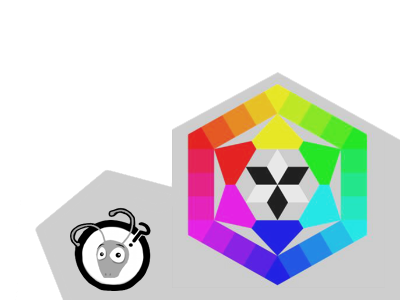
\includegraphics[width=0.2\textwidth]{png/menu.png}\ 
	Der Farbkreis zeigt den aktuellen Fortschritt an. Zu Beginn des Spiels ist er komplett grau, mit jeder neu erworbenen Farbe füllt sich der Kreis langsam.\\
	Links daneben befindet sich das Motten-Symbol. Über dieses können nützliche Hinweise zum aktuellen Level abgerufen werden. Die Motte erklärt dabei die 		theoretischen Grundlagen die für die Bewältigung dieses Levels von Bedeutung sind.\\\\
	Bei einem Klick öffnet sich ein neues Fenster:\\\\
	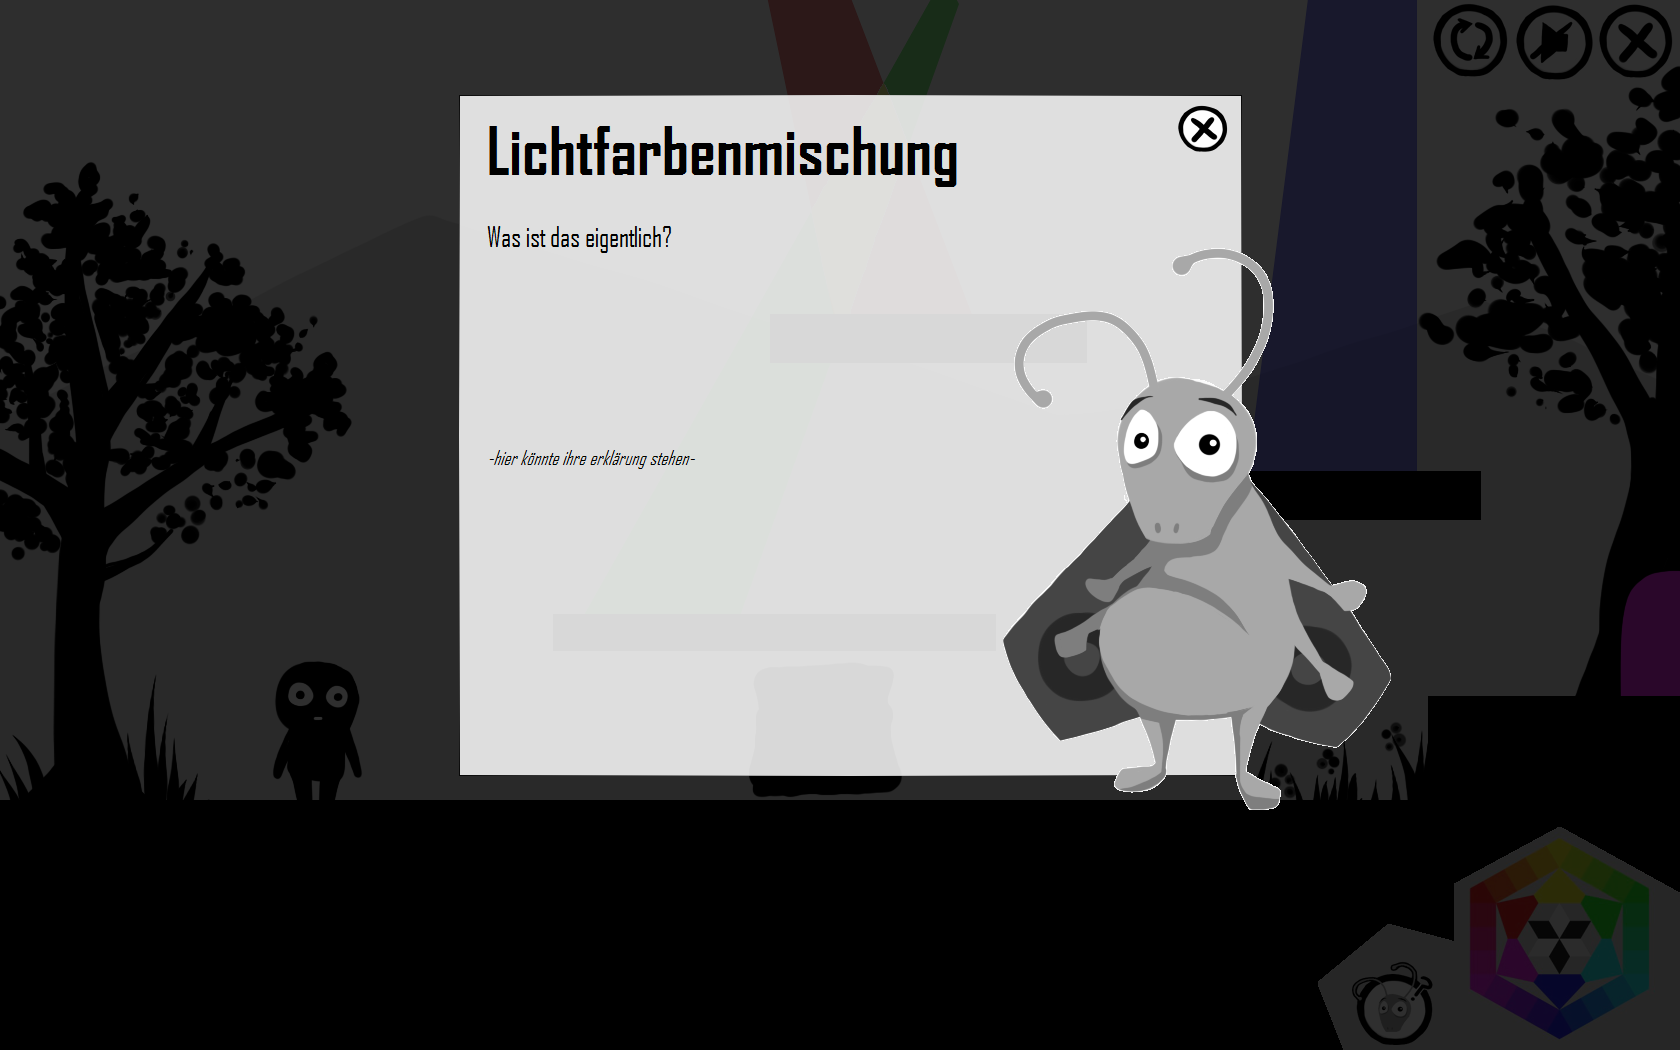
\includegraphics[width=1\textwidth]{png/screen_help.png}\ 
	\\
	\clearpage\
	\\
	\Zwei{Levelübersicht}\\
	\\
	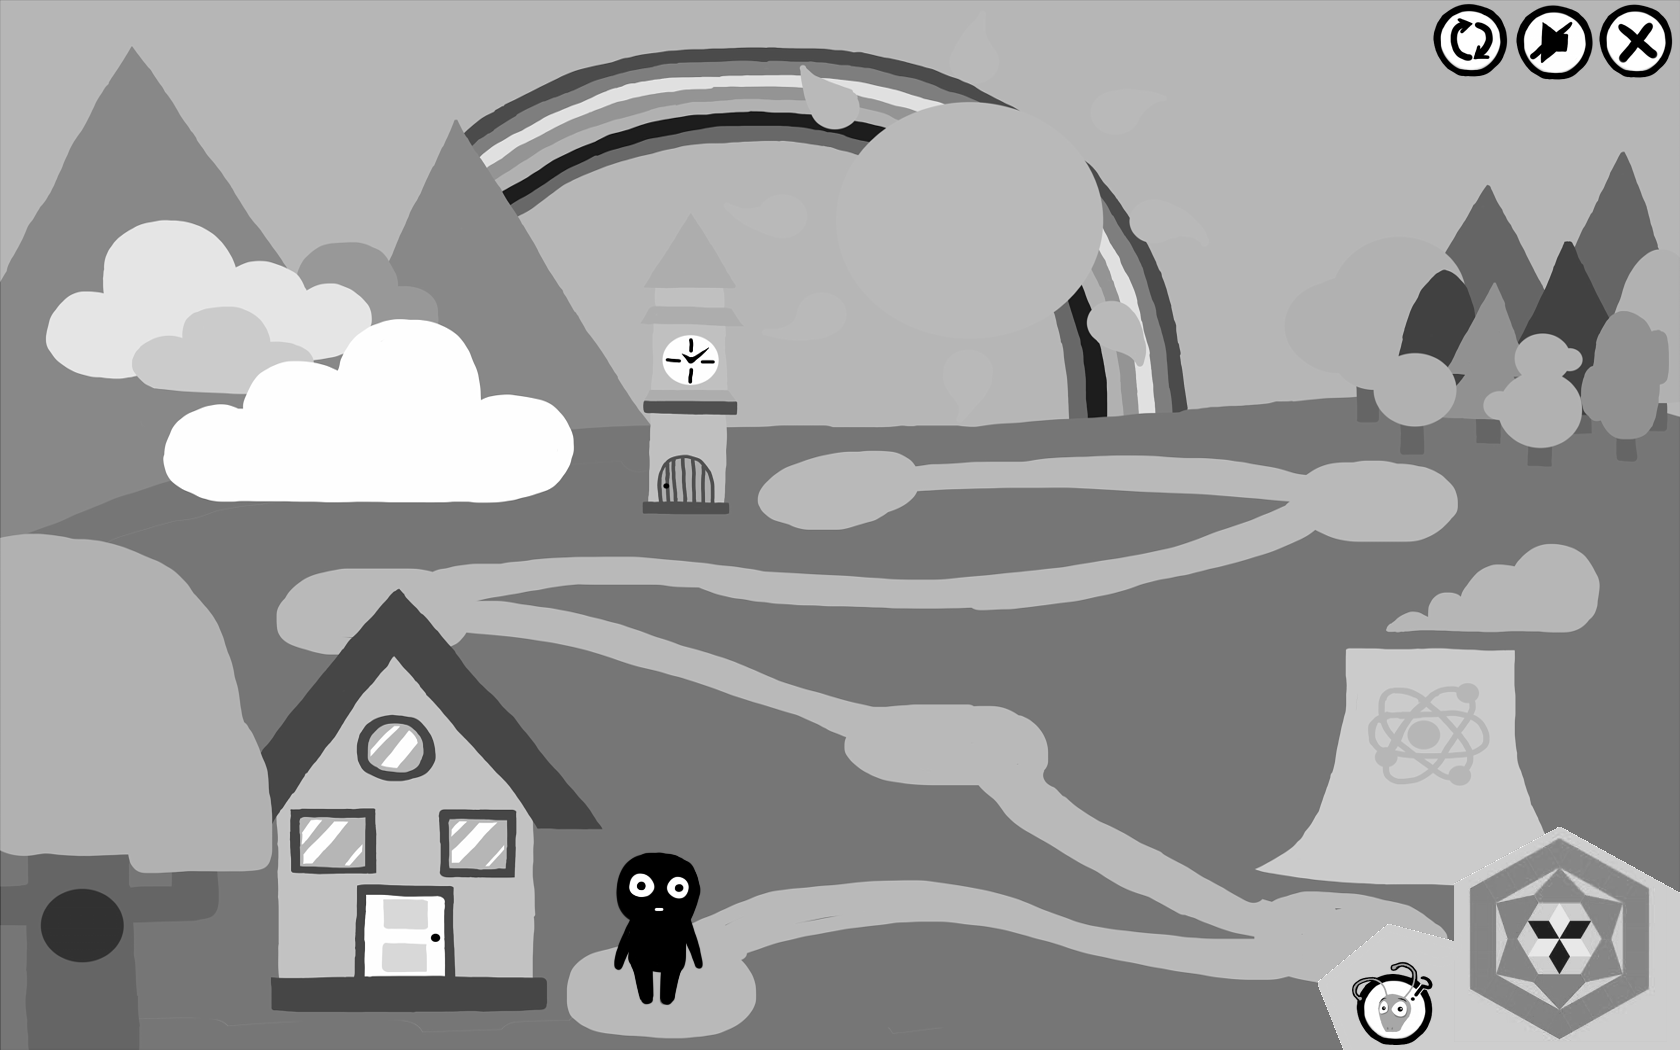
\includegraphics[width=1\textwidth]{png/screen_overview.png}\
	\\\\
	\Text
	Dies ist die Levelübersicht. Nach Absolvierung jedes Levels findet sich der Spieler hier wieder. Die Landschaft färbt sich dabei proportional zum Spielfortschritt 		ein. Hier zu sehen ist demnach der Spielstart.\\
	Die einzelnen Level bewegen sich anhand des eingezeichneten Pfads. Die Umgebung an den Stationen gibt Hinweise auf den Inhalt des Levels. 
	So ist auch in den Level die Struktur der Welt präsent.
	\clearpage\
	\\
	\Zwei{Beispiel eines Levels}\\
	\\
	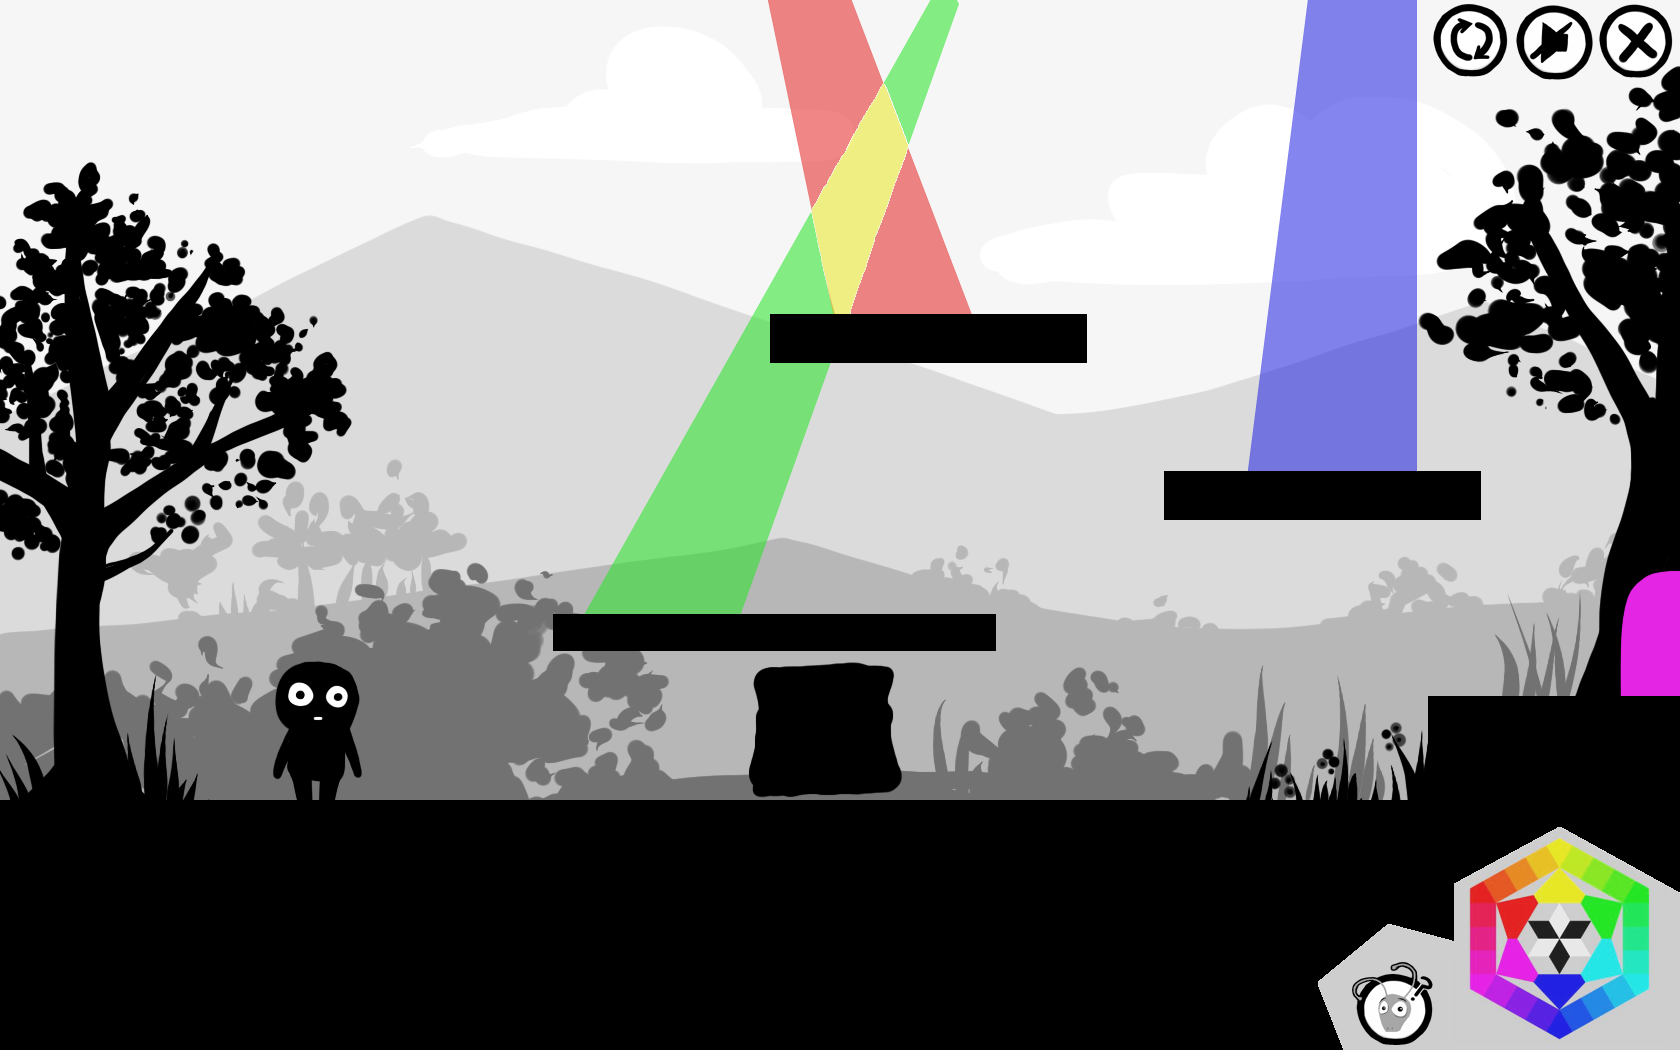
\includegraphics[width=1\textwidth]{png/screen.png}\
	\\\\
	\Text
	Beispielhafte Darstellung eines Levels, hier nur unter Einbindung der Lichtfarbenmischung. Die tatsächlichen Level sind umfangreicher und länger,
	dies sei nur eine Skizze zur Veranschaulichung.\\\\
	Charakter und begehbare Stage sind dabei stets in schwarz gehalten, der Hintergrund schließt sich in Grautönen an.\\
	Die Lichtkegel und das Tor dass mit Beendigung des Level durchschritten werden muss sind bunt. In dem Level können sich jedoch auch weitere
	Interaktionsmöglichkeiten befinden, hier in Form eines Felsens der verschoben werden muss.
	\\\\
	\\\\
	\Fusszeile
\end{document}